\section{Theoretical Analysis}
\label{sec:analysis}


\subsection{1}

%First Matrix
$\begin{pmatrix}
1 & 0 & 0 & -1 & 0 & 0 & 0 & 0\\
-G1 & G1+G2+G3 & -G2 & 0 & -G3 & 0 & 0 & 0\\
0 & -G2-Kb & G2 & 0 & Kb & 0 & 0 & 0 \\
G1 & -G1 & 0 & G4+G6 & -G4 & 0 & -G6 & 0\\
0 & 0 & 0 & -Kd*G6 & 1 & 0 & Kd*G6 & 0 \\
0 & Kb & 0 & 0 & -G5-Kb & G5 & 0 & 0 \\
0 & 0 & 0 & -G6 & 0 & 0 & G6+G7 & 0  \\ 
0 & 0 & 0 & 1 & 0 & 0 & 0 & 0
\end{pmatrix}$
$\begin{pmatrix}
V1\\
V2\\
V3\\
V4\\
V5\\
V6\\
V7\\
V8
\end{pmatrix}$
=
$\begin{pmatrix}
V5\\
0\\
0\\
0\\
0\\
0\\
0\\
0
\end{pmatrix}$

%Table(tensoes_tab) 
\begin{table}[H] \centering
\begin{tabular}{|
>{\columncolor[HTML]{FFCC67}}l |c|}
\hline
\multicolumn{2}{|l|}{\cellcolor[HTML]{EABD8B}Octave - Voltages (V)} \\ \hline
{\color[HTML]{333333} V1}               & 5.216040e+00               \\ \hline
{\color[HTML]{333333} V2}               & 4.939074e+00               \\ \hline
{\color[HTML]{333333} V3}               & 4.361415e+00               \\ \hline
{\color[HTML]{333333} V4}               & 0.000000e+00              \\ \hline
{\color[HTML]{333333} V5}               & 4.978786e+00               \\ \hline
{\color[HTML]{333333} V6}               & 5.853598e+00               \\ \hline
{\color[HTML]{333333} V7}               & -2.001094e+00              \\ \hline
{\color[HTML]{333333} V8}               & -2.978754e+00              \\ \hline
\end{tabular}
\caption{Octave solution (Voltages)}
\end{table}



\subsection{2}

%Second Matrix
$\begin{pmatrix}
0 & 0 & 0 & 0 & 0 & 1 & 0 & -1\\
-G1 & G1+G2+G3 & -G2 & 0 & -G3 & 0 & 0 & 0\\
0 & -G2-Kb & G2 & 0 & Kb & 0 & 0 & 0 \\
G1 & -G1 & 0 & G4+G6 & -G4 & 0 & -G6 & 0\\
0 & 0 & 0 & -Kd*G6 & 1 & 0 & Kd*G6 & 0 \\
1 & 0 & 0 & -1 & 0 & 0 & 0 & 0\\
0 & 0 & 0 & -G6 & 0 & 0 & G6+G7 & -G7  \\ 
0 & 0 & 0 & 1 & 0 & 0 & 0 & 0
\end{pmatrix}$
$\begin{pmatrix}
V1\\
V2\\
V3\\
V4\\
V5\\
V6\\
V7\\
V8
\end{pmatrix}$
=
$\begin{pmatrix}
Vx\\
0\\
0\\
0\\
0\\
0\\
0\\
0
\end{pmatrix}$

%Table (R_eq)
\begin{table}[H] \centering
\begin{tabular}{|
>{\columncolor[HTML]{FFCC67}}l |c|}
\hline
\multicolumn{2}{|l|}{\cellcolor[HTML]{EABD8B}$R_{eq}$ ($\Omega$)} \\ \hline
{\color[HTML]{333333} $R_{eq}$}           &  -1.316042e-03        \\ \hline
\end{tabular}
\caption{Octave solution ($R_{eq}$)}
\end{table}

\subsection{3}

%plot do natural

\begin{figure}[H]
\centering
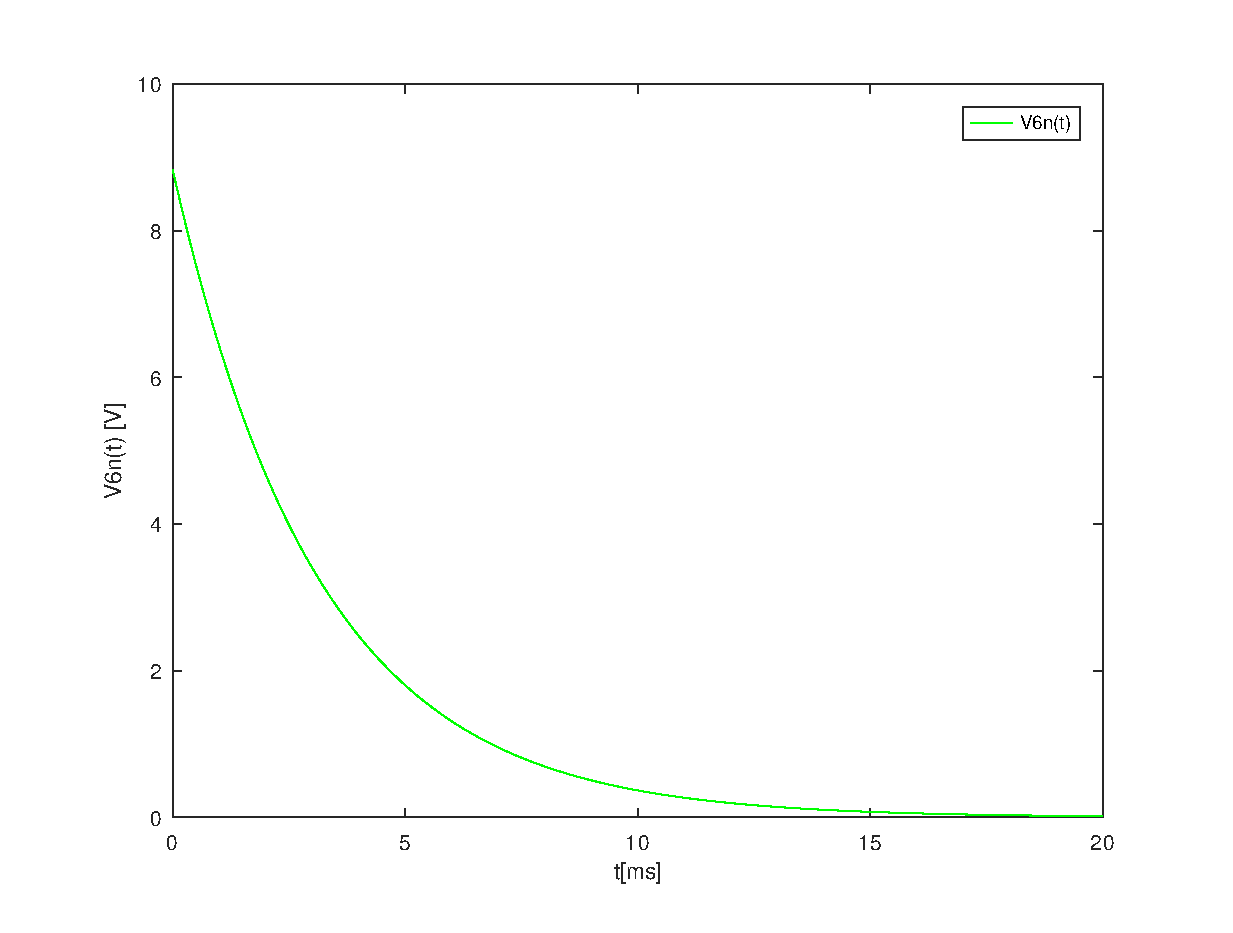
\includegraphics[width = 15cm]{NaturalResponse.eps}
\caption {Natural Response}
\end{figure}

\begin{figure}[H]
\centering
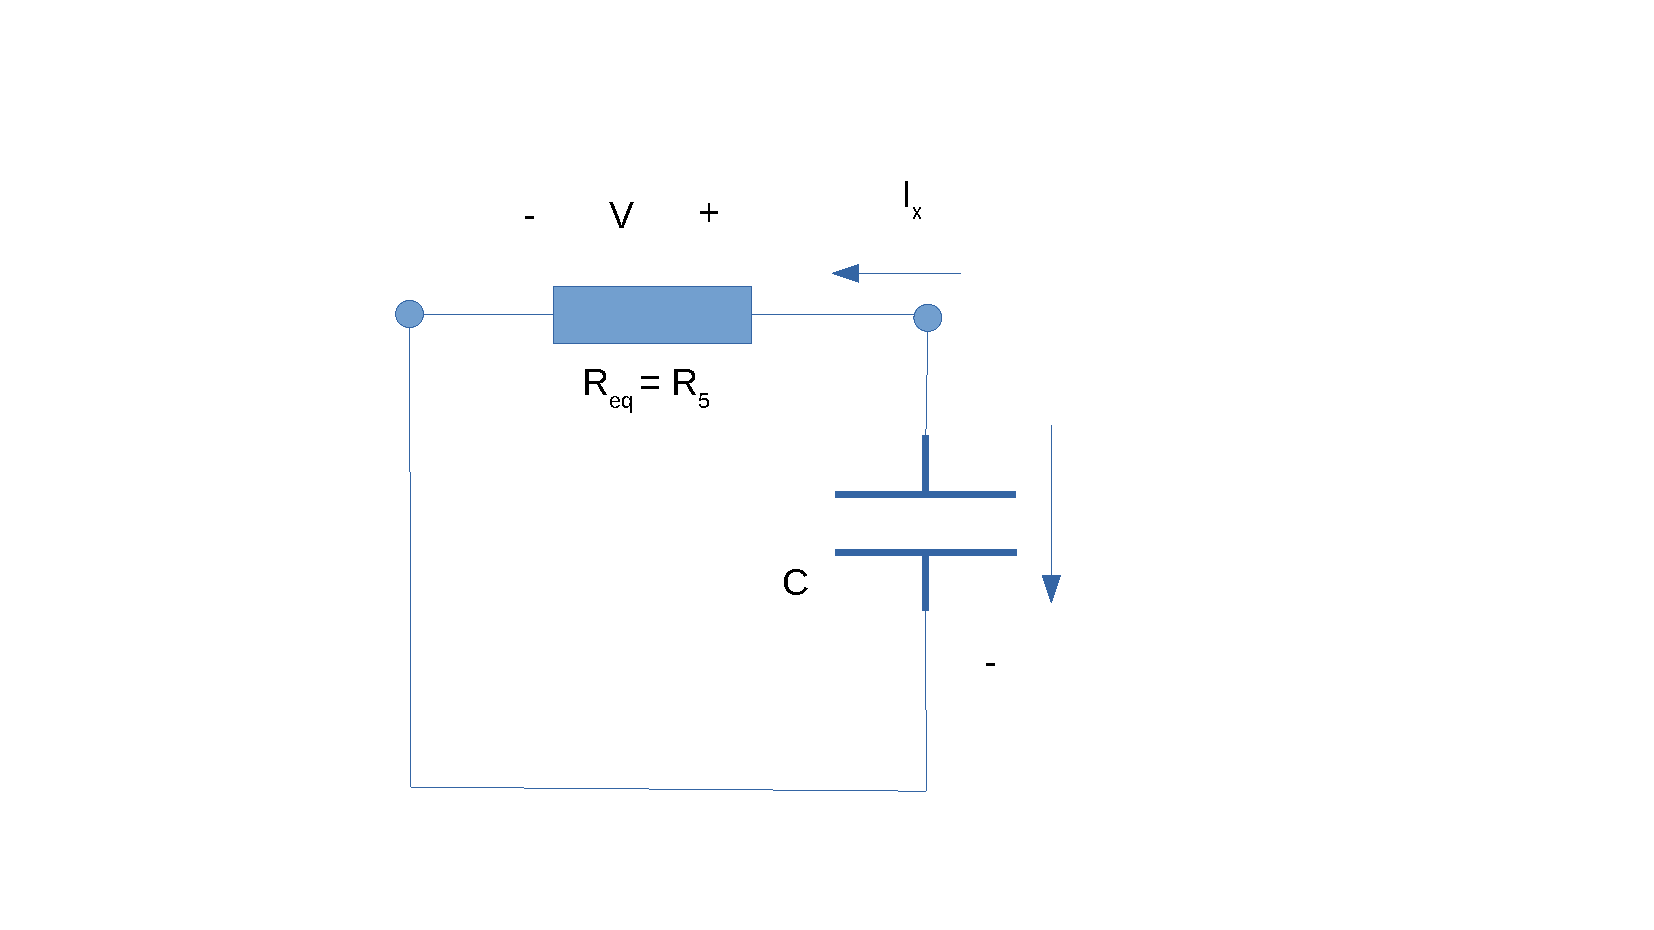
\includegraphics[width = 15cm]{circuit3.pdf}
\caption {Circuit3}
\end{figure}

\subsection{4} 

%Tabela com complexos 
\begin{table}[H] \centering
\begin{tabular}{|
>{\columncolor[HTML]{FFCC67}}l |c|}
\hline
\multicolumn{2}{|l|}{\cellcolor[HTML]{EABD8B}Complex Amplitudes(V)} \\ \hline
{\color[HTML]{333333} V1}               & 1.000000e+00 + i(-1.549812e-33)               \\ \hline
{\color[HTML]{333333} V2}               & 9.469010e-01 + i(-1.466518e-17)               \\ \hline
{\color[HTML]{333333} V3}               & 8.361543e-01 + i(5.184518e-16)               \\ \hline
{\color[HTML]{333333} V4}               & 0.000000e+00 + i(-1.549812e-33)              \\ \hline
{\color[HTML]{333333} V5}               & 9.545144e-01 + i(-5.131501e-17)              \\ \hline
{\color[HTML]{333333} V6}               & -5.667484e-01 + i(-8.549146e-02)               \\ \hline
{\color[HTML]{333333} V7}               & -3.836423e-01 + i(2.062473e-17)              \\ \hline
{\color[HTML]{333333} V8}               & -5.710758e-01 + i(3.070122e-17)             \\ \hline
\end{tabular}
\caption{Octave solution (Complex Amplitudes)}
\end{table}



%Se precisares
\begin{figure}[H]
\centering
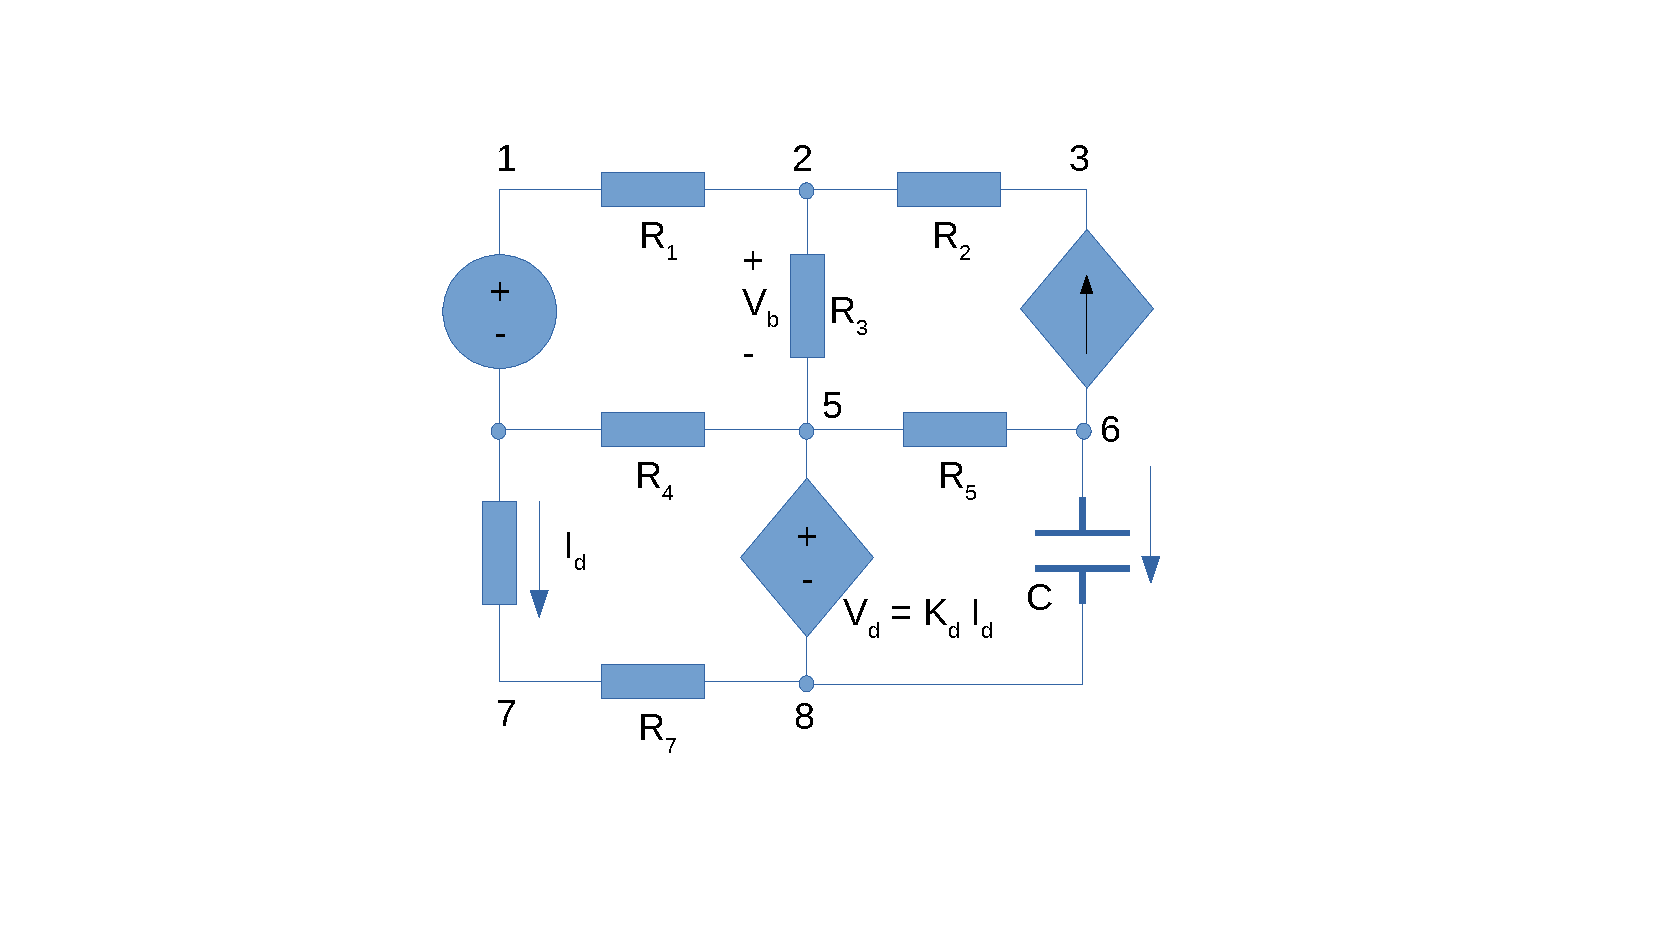
\includegraphics[width = 15cm]{circuit1.pdf}
\caption {Circuit1}
\end{figure}

%Third Matrix
$\begin{pmatrix}
1 & 0 & 0 & -1 & 0 & 0 & 0 & 0\\
-G1 & G1+G2+G3 & -G2 & 0 & -G3 & 0 & 0 & 0\\
0 & -G2-Kb & G2 & 0 & Kb & 0 & 0 & 0 \\
G1 & -G1 & 0 & G4+G6 & -G4 & 0 & -G6 & 0\\
0 & 0 & 0 & -Kd*G6 & 1 & 0 & Kd*G6 & -1 \\
0 & Kb & 0 & 0 & -G5-Kb & G5+\frac{1}{Z_c} & 0 & -\frac{1}{Z_c} \\
0 & 0 & 0 & -G6 & 0 & 0 & G6+G7 & -G7  \\ 
0 & 0 & 0 & 1 & 0 & 0 & 0 & 0
\end{pmatrix}$
$\begin{pmatrix}
V1\\
V2\\
V3\\
V4\\
V5\\
V6\\
V7\\
V8
\end{pmatrix}$
=
$\begin{pmatrix}
V_s(t)\\
0\\
0\\
0\\
0\\
0\\
0\\
0
\end{pmatrix}$

\subsection{5}

%Plot de ambos
\begin{figure}[H]
\centering
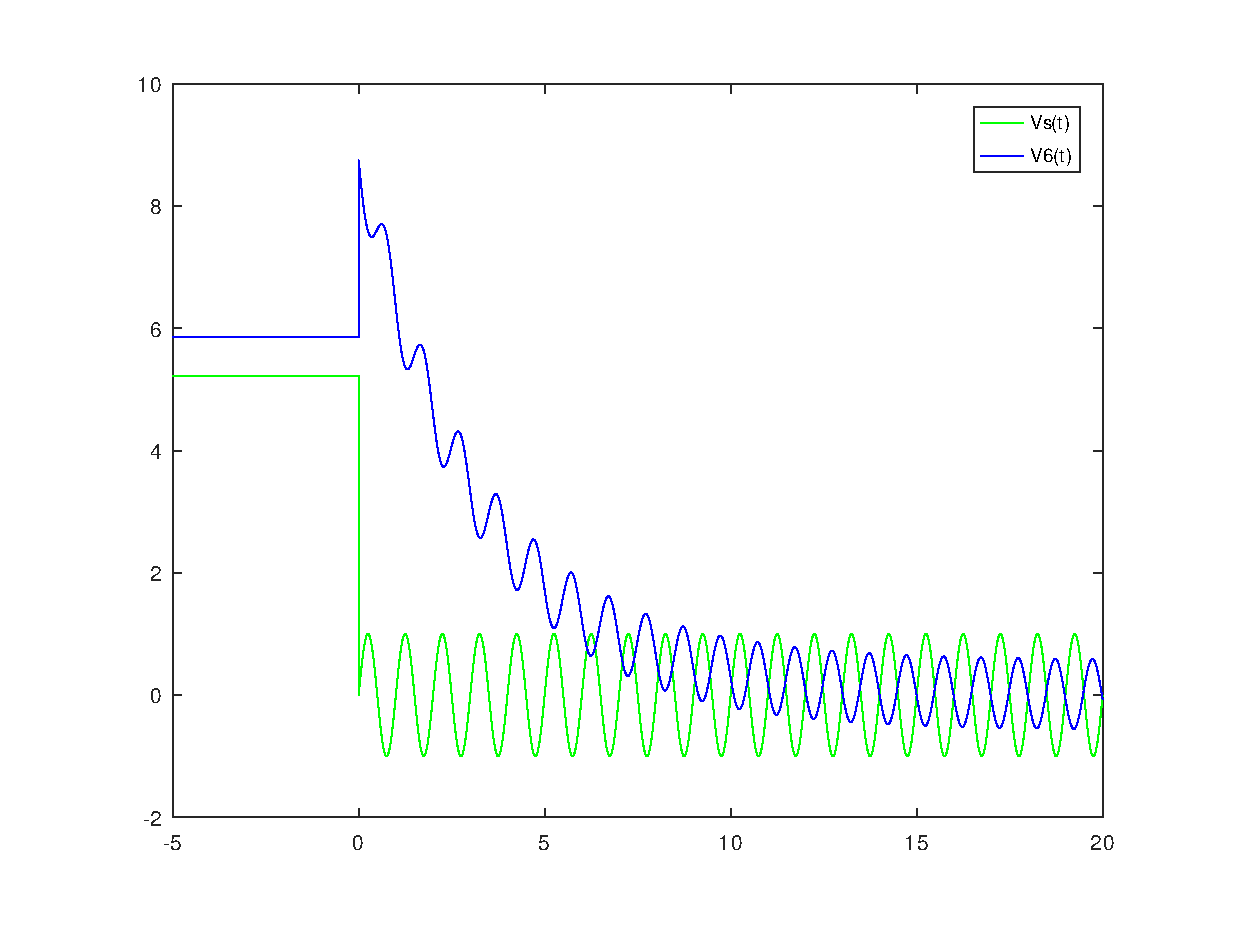
\includegraphics[width = 15cm]{Solution.eps}
\caption {Natural and forced response}
\end{figure}

%V6(t)
%\begin{equation}
 %V_{6}(t)=
  %  \begin{cases}
   %   V_{6i} & \text{para t $\in$ [-5, 0]}\\
    %  V_{6n}(t) + V_{6f}(t) = V_{6i}e^{$\frac{t}{C*R_5}$} + Acos($\omega$ t - $\phi$_1)
    %\end{cases}       
%\end{equation}


\subsection{6}

%plot 
\begin{figure}[H]
\centering
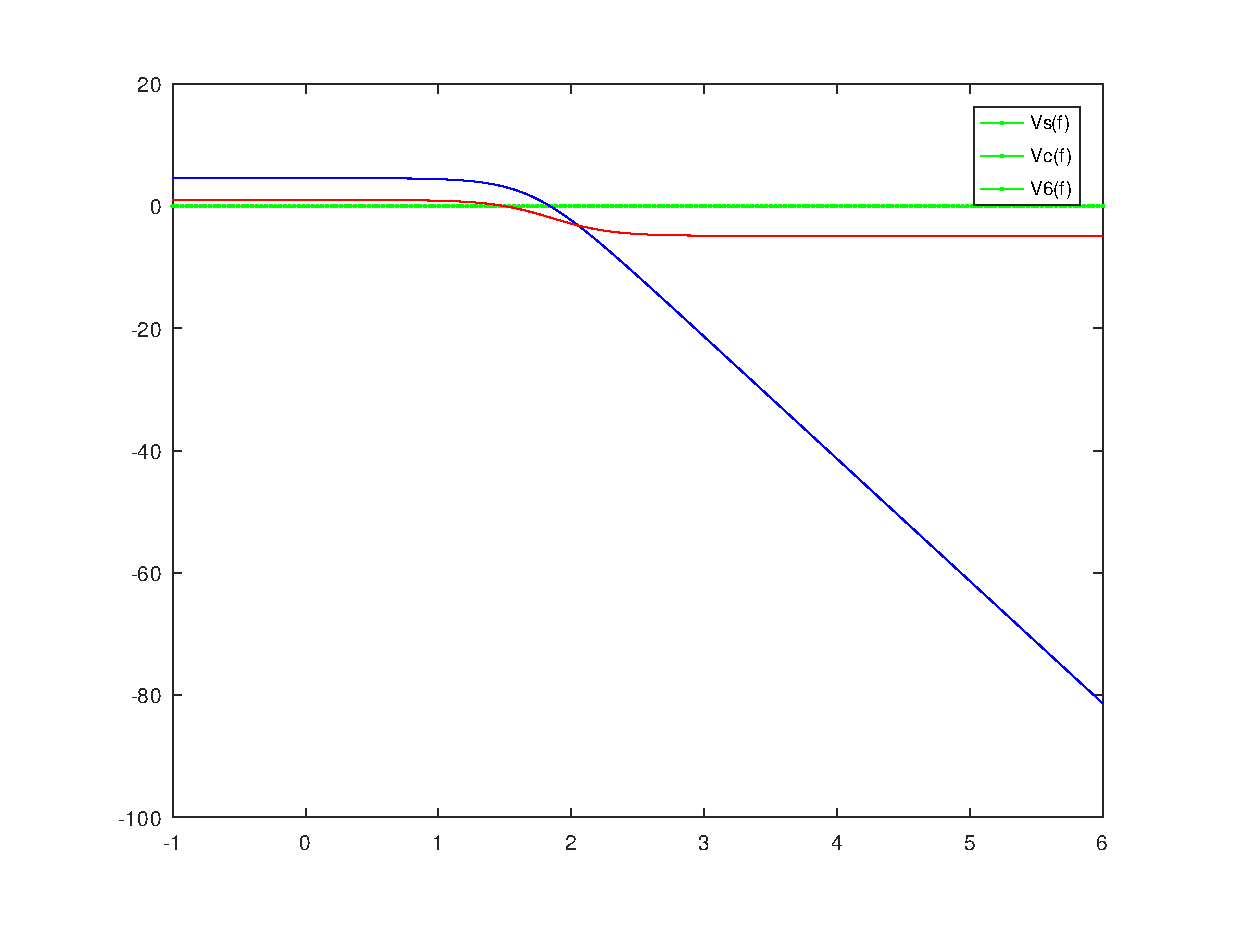
\includegraphics[width = 15cm]{Amplitude.eps}
\caption {Amplitude}
\end{figure}

\begin{figure}[H]
\centering
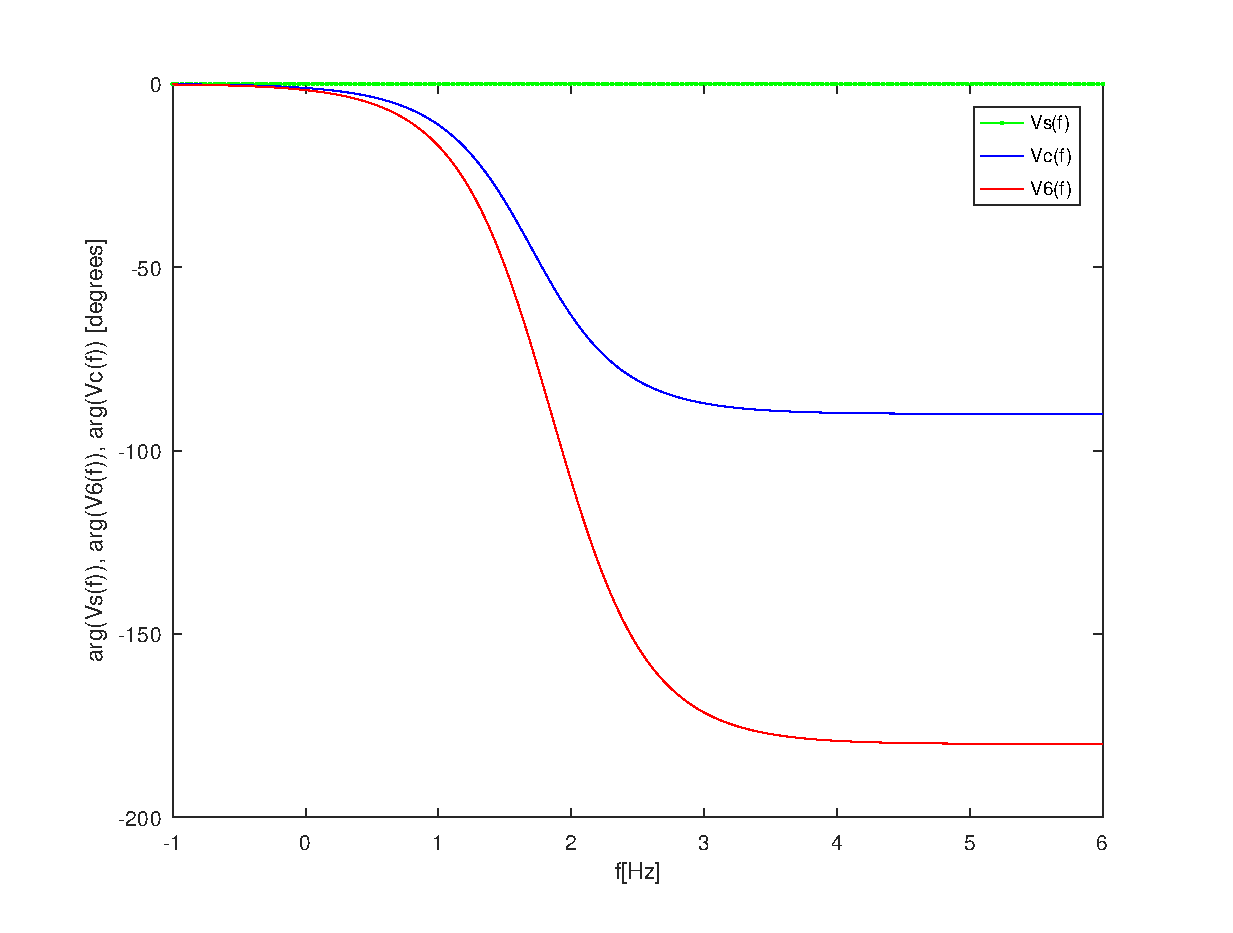
\includegraphics[width = 15cm]{Arguments.eps}
\caption {Arguments}
\end{figure}

